% Created by tikzDevice version 0.7.0 on 2015-06-28 00:48:39
% !TEX encoding = UTF-8 Unicode
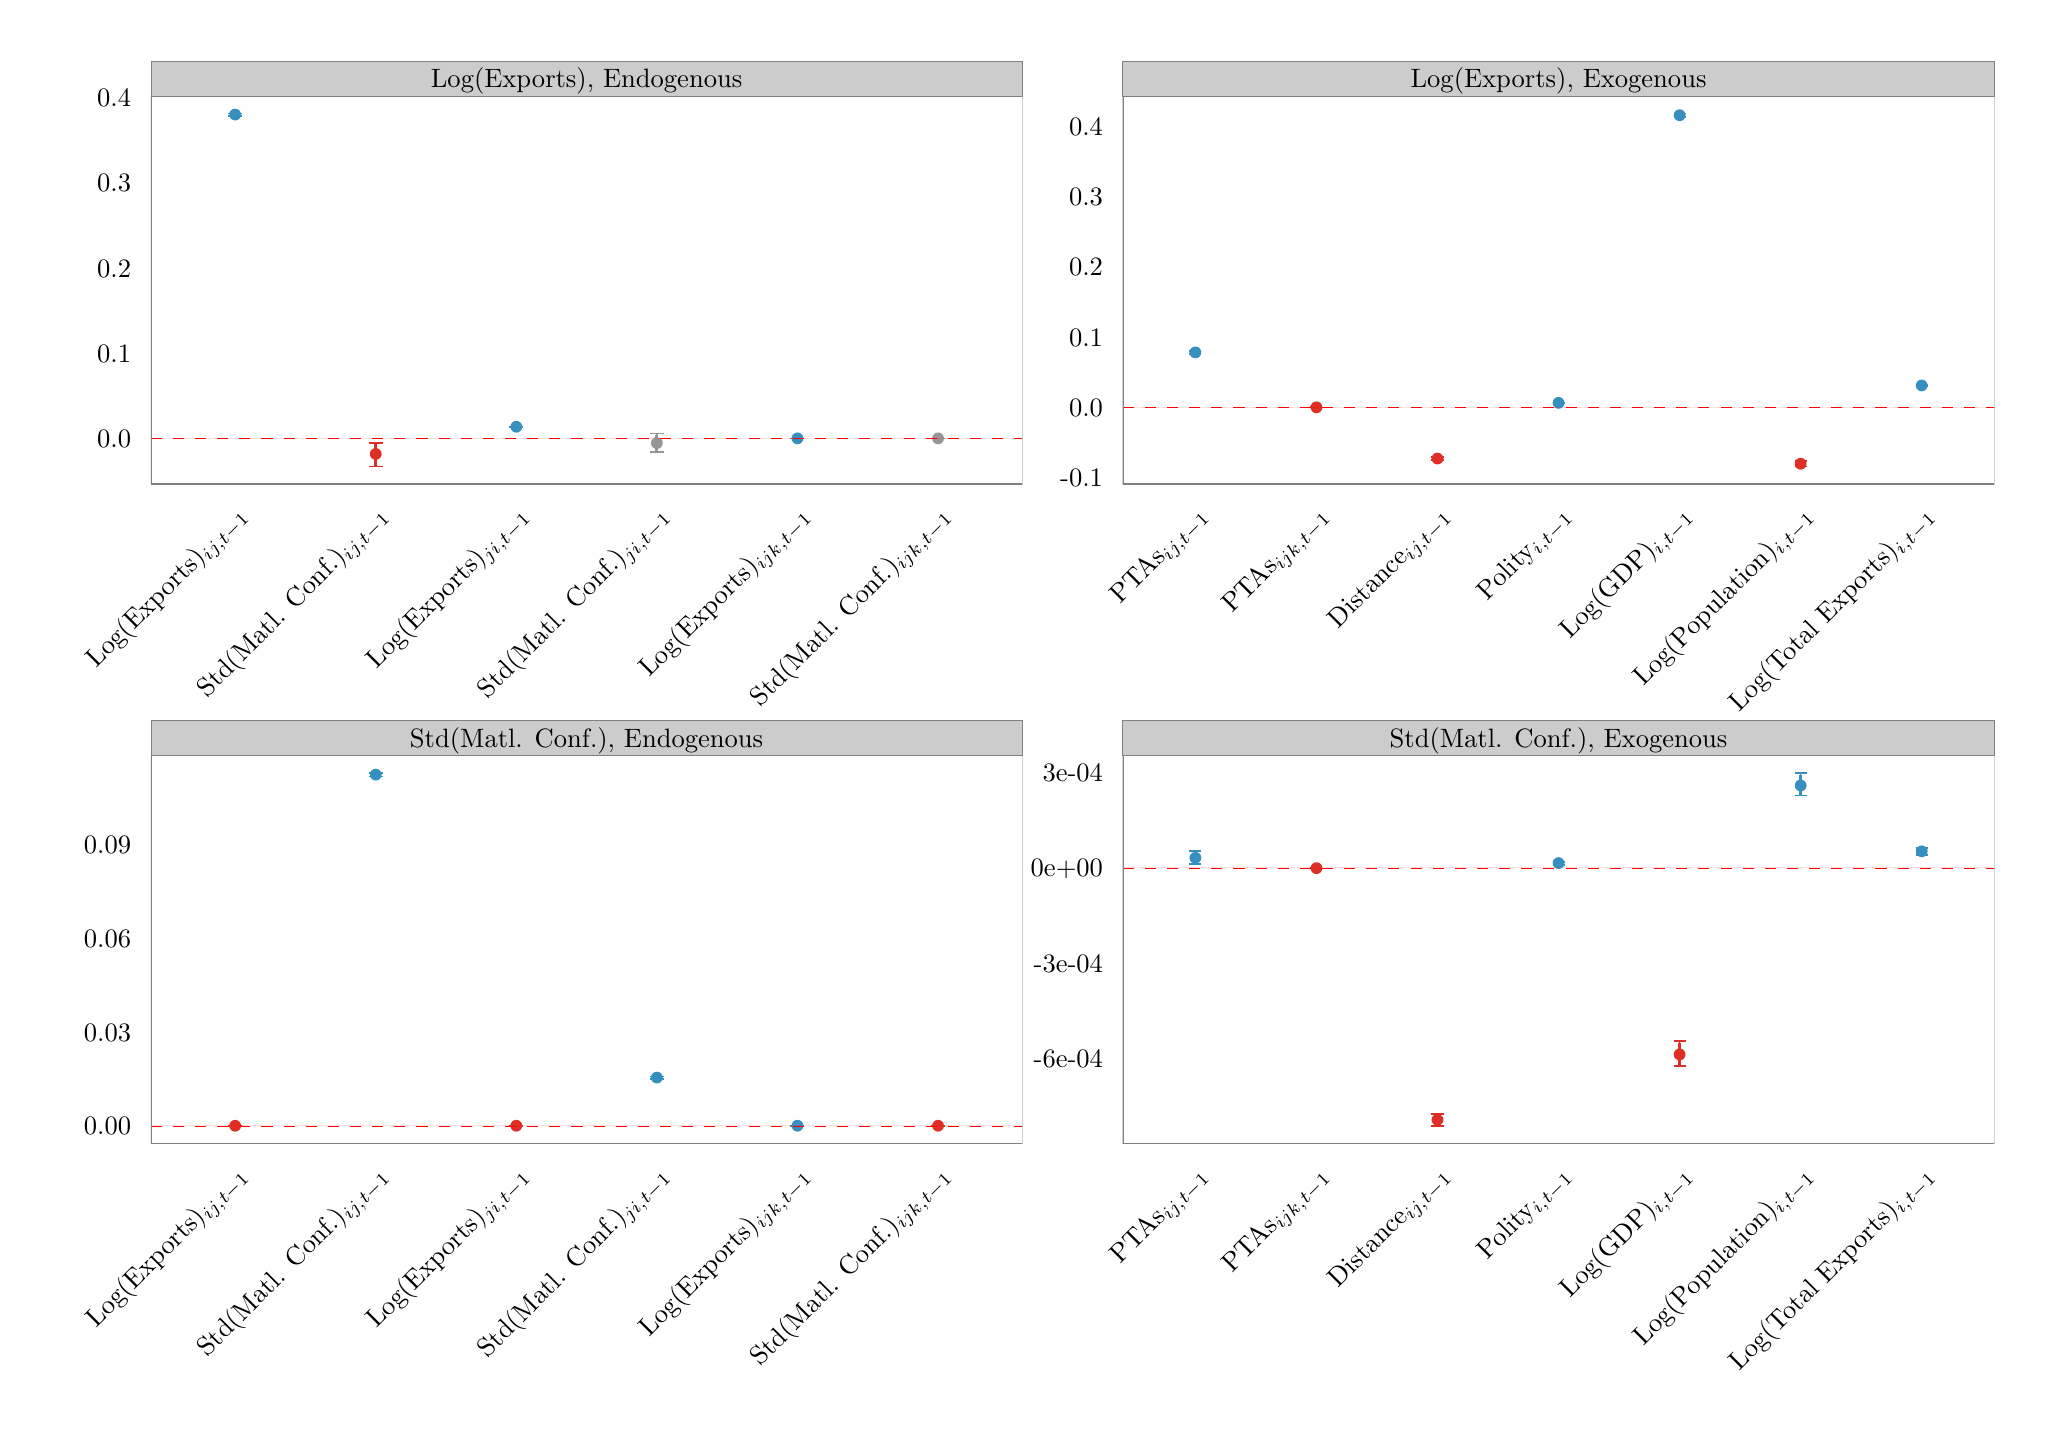
\begin{tikzpicture}[x=1pt,y=1pt]
\definecolor[named]{fillColor}{rgb}{1.00,1.00,1.00}
\path[use as bounding box,fill=fillColor,fill opacity=0.00] (0,0) rectangle (722.70,505.89);
\begin{scope}
\path[clip] (  0.00,  0.00) rectangle (722.70,505.89);
\definecolor[named]{drawColor}{rgb}{1.00,1.00,1.00}
\definecolor[named]{fillColor}{rgb}{1.00,1.00,1.00}

\path[draw=drawColor,line width= 0.6pt,line join=round,line cap=round,fill=fillColor] (  0.00,  0.00) rectangle (722.70,505.89);
\end{scope}
\begin{scope}
\path[clip] ( 44.49,340.99) rectangle (359.44,481.21);
\definecolor[named]{fillColor}{rgb}{0.21,0.56,0.75}

\path[fill=fillColor] ( 74.97,474.48) circle (  2.13);
\definecolor[named]{fillColor}{rgb}{0.87,0.18,0.15}

\path[fill=fillColor] (125.77,351.85) circle (  2.13);
\definecolor[named]{fillColor}{rgb}{0.21,0.56,0.75}

\path[fill=fillColor] (176.56,361.68) circle (  2.13);
\definecolor[named]{fillColor}{rgb}{0.59,0.59,0.59}

\path[fill=fillColor] (227.36,355.77) circle (  2.13);
\definecolor[named]{fillColor}{rgb}{0.21,0.56,0.75}

\path[fill=fillColor] (278.16,357.48) circle (  2.13);
\definecolor[named]{fillColor}{rgb}{0.59,0.59,0.59}

\path[fill=fillColor] (328.96,357.48) circle (  2.13);
\definecolor[named]{drawColor}{rgb}{0.21,0.56,0.75}
\definecolor[named]{fillColor}{rgb}{0.21,0.56,0.75}

\path[draw=drawColor,draw opacity=0.30,line width= 0.3pt,line join=round,fill=fillColor,fill opacity=0.30] ( 74.97,474.04) -- ( 74.97,474.84);
\definecolor[named]{drawColor}{rgb}{0.87,0.18,0.15}
\definecolor[named]{fillColor}{rgb}{0.87,0.18,0.15}

\path[draw=drawColor,draw opacity=0.30,line width= 0.3pt,line join=round,fill=fillColor,fill opacity=0.30] (125.77,347.36) -- (125.77,355.83);
\definecolor[named]{drawColor}{rgb}{0.21,0.56,0.75}
\definecolor[named]{fillColor}{rgb}{0.21,0.56,0.75}

\path[draw=drawColor,draw opacity=0.30,line width= 0.3pt,line join=round,fill=fillColor,fill opacity=0.30] (176.56,361.58) -- (176.56,361.78);
\definecolor[named]{drawColor}{rgb}{0.59,0.59,0.59}
\definecolor[named]{fillColor}{rgb}{0.59,0.59,0.59}

\path[draw=drawColor,draw opacity=0.30,line width= 0.3pt,line join=round,fill=fillColor,fill opacity=0.30] (227.36,352.62) -- (227.36,359.22);
\definecolor[named]{drawColor}{rgb}{0.21,0.56,0.75}
\definecolor[named]{fillColor}{rgb}{0.21,0.56,0.75}

\path[draw=drawColor,draw opacity=0.30,line width= 0.3pt,line join=round,fill=fillColor,fill opacity=0.30] (278.16,357.48) -- (278.16,357.48);
\definecolor[named]{drawColor}{rgb}{0.59,0.59,0.59}
\definecolor[named]{fillColor}{rgb}{0.59,0.59,0.59}

\path[draw=drawColor,draw opacity=0.30,line width= 0.3pt,line join=round,fill=fillColor,fill opacity=0.30] (328.96,357.47) -- (328.96,357.49);
\definecolor[named]{drawColor}{rgb}{0.21,0.56,0.75}
\definecolor[named]{fillColor}{rgb}{0.21,0.56,0.75}

\path[draw=drawColor,line width= 1.1pt,line join=round,fill=fillColor] ( 74.97,474.14) -- ( 74.97,474.80);
\definecolor[named]{drawColor}{rgb}{0.87,0.18,0.15}
\definecolor[named]{fillColor}{rgb}{0.87,0.18,0.15}

\path[draw=drawColor,line width= 1.1pt,line join=round,fill=fillColor] (125.77,347.57) -- (125.77,355.40);
\definecolor[named]{drawColor}{rgb}{0.21,0.56,0.75}
\definecolor[named]{fillColor}{rgb}{0.21,0.56,0.75}

\path[draw=drawColor,line width= 1.1pt,line join=round,fill=fillColor] (176.56,361.60) -- (176.56,361.76);
\definecolor[named]{drawColor}{rgb}{0.59,0.59,0.59}
\definecolor[named]{fillColor}{rgb}{0.59,0.59,0.59}

\path[draw=drawColor,line width= 1.1pt,line join=round,fill=fillColor] (227.36,353.08) -- (227.36,358.67);
\definecolor[named]{drawColor}{rgb}{0.21,0.56,0.75}
\definecolor[named]{fillColor}{rgb}{0.21,0.56,0.75}

\path[draw=drawColor,line width= 1.1pt,line join=round,fill=fillColor] (278.16,357.48) -- (278.16,357.48);
\definecolor[named]{drawColor}{rgb}{0.59,0.59,0.59}
\definecolor[named]{fillColor}{rgb}{0.59,0.59,0.59}

\path[draw=drawColor,line width= 1.1pt,line join=round,fill=fillColor] (328.96,357.47) -- (328.96,357.49);
\definecolor[named]{drawColor}{rgb}{0.21,0.56,0.75}

\path[draw=drawColor,line width= 0.6pt,line join=round] ( 72.43,474.84) --
	( 77.51,474.84);

\path[draw=drawColor,line width= 0.6pt,line join=round] ( 74.97,474.84) --
	( 74.97,474.04);

\path[draw=drawColor,line width= 0.6pt,line join=round] ( 72.43,474.04) --
	( 77.51,474.04);
\definecolor[named]{drawColor}{rgb}{0.87,0.18,0.15}

\path[draw=drawColor,line width= 0.6pt,line join=round] (123.23,355.83) --
	(128.31,355.83);

\path[draw=drawColor,line width= 0.6pt,line join=round] (125.77,355.83) --
	(125.77,347.36);

\path[draw=drawColor,line width= 0.6pt,line join=round] (123.23,347.36) --
	(128.31,347.36);
\definecolor[named]{drawColor}{rgb}{0.21,0.56,0.75}

\path[draw=drawColor,line width= 0.6pt,line join=round] (174.03,361.78) --
	(179.10,361.78);

\path[draw=drawColor,line width= 0.6pt,line join=round] (176.56,361.78) --
	(176.56,361.58);

\path[draw=drawColor,line width= 0.6pt,line join=round] (174.03,361.58) --
	(179.10,361.58);
\definecolor[named]{drawColor}{rgb}{0.59,0.59,0.59}

\path[draw=drawColor,line width= 0.6pt,line join=round] (224.82,359.22) --
	(229.90,359.22);

\path[draw=drawColor,line width= 0.6pt,line join=round] (227.36,359.22) --
	(227.36,352.62);

\path[draw=drawColor,line width= 0.6pt,line join=round] (224.82,352.62) --
	(229.90,352.62);
\definecolor[named]{drawColor}{rgb}{0.21,0.56,0.75}

\path[draw=drawColor,line width= 0.6pt,line join=round] (275.62,357.48) --
	(280.70,357.48);

\path[draw=drawColor,line width= 0.6pt,line join=round] (278.16,357.48) --
	(278.16,357.48);

\path[draw=drawColor,line width= 0.6pt,line join=round] (275.62,357.48) --
	(280.70,357.48);
\definecolor[named]{drawColor}{rgb}{0.59,0.59,0.59}

\path[draw=drawColor,line width= 0.6pt,line join=round] (326.42,357.49) --
	(331.50,357.49);

\path[draw=drawColor,line width= 0.6pt,line join=round] (328.96,357.49) --
	(328.96,357.47);

\path[draw=drawColor,line width= 0.6pt,line join=round] (326.42,357.47) --
	(331.50,357.47);
\definecolor[named]{drawColor}{rgb}{1.00,0.00,0.00}
\definecolor[named]{fillColor}{rgb}{1.00,0.00,0.00}

\path[draw=drawColor,line width= 0.1pt,dash pattern=on 4pt off 4pt ,line join=round,fill=fillColor] ( 44.49,357.47) -- (359.44,357.47);
\definecolor[named]{drawColor}{rgb}{0.50,0.50,0.50}

\path[draw=drawColor,line width= 0.6pt,line join=round,line cap=round] ( 44.49,340.99) rectangle (359.44,481.21);
\end{scope}
\begin{scope}
\path[clip] (395.70,340.99) rectangle (710.66,481.21);
\definecolor[named]{fillColor}{rgb}{0.21,0.56,0.75}

\path[fill=fillColor] (421.94,388.54) circle (  2.13);
\definecolor[named]{fillColor}{rgb}{0.87,0.18,0.15}

\path[fill=fillColor] (465.69,368.70) circle (  2.13);

\path[fill=fillColor] (509.43,350.19) circle (  2.13);
\definecolor[named]{fillColor}{rgb}{0.21,0.56,0.75}

\path[fill=fillColor] (553.18,370.30) circle (  2.13);

\path[fill=fillColor] (596.92,474.24) circle (  2.13);
\definecolor[named]{fillColor}{rgb}{0.87,0.18,0.15}

\path[fill=fillColor] (640.66,348.31) circle (  2.13);
\definecolor[named]{fillColor}{rgb}{0.21,0.56,0.75}

\path[fill=fillColor] (684.41,376.60) circle (  2.13);
\definecolor[named]{drawColor}{rgb}{0.21,0.56,0.75}
\definecolor[named]{fillColor}{rgb}{0.21,0.56,0.75}

\path[draw=drawColor,draw opacity=0.30,line width= 0.3pt,line join=round,fill=fillColor,fill opacity=0.30] (421.94,388.08) -- (421.94,389.13);
\definecolor[named]{drawColor}{rgb}{0.87,0.18,0.15}
\definecolor[named]{fillColor}{rgb}{0.87,0.18,0.15}

\path[draw=drawColor,draw opacity=0.30,line width= 0.3pt,line join=round,fill=fillColor,fill opacity=0.30] (465.69,368.69) -- (465.69,368.70);

\path[draw=drawColor,draw opacity=0.30,line width= 0.3pt,line join=round,fill=fillColor,fill opacity=0.30] (509.43,349.63) -- (509.43,350.86);
\definecolor[named]{drawColor}{rgb}{0.21,0.56,0.75}
\definecolor[named]{fillColor}{rgb}{0.21,0.56,0.75}

\path[draw=drawColor,draw opacity=0.30,line width= 0.3pt,line join=round,fill=fillColor,fill opacity=0.30] (553.18,370.18) -- (553.18,370.40);

\path[draw=drawColor,draw opacity=0.30,line width= 0.3pt,line join=round,fill=fillColor,fill opacity=0.30] (596.92,473.68) -- (596.92,474.84);
\definecolor[named]{drawColor}{rgb}{0.87,0.18,0.15}
\definecolor[named]{fillColor}{rgb}{0.87,0.18,0.15}

\path[draw=drawColor,draw opacity=0.30,line width= 0.3pt,line join=round,fill=fillColor,fill opacity=0.30] (640.66,347.36) -- (640.66,349.30);
\definecolor[named]{drawColor}{rgb}{0.21,0.56,0.75}
\definecolor[named]{fillColor}{rgb}{0.21,0.56,0.75}

\path[draw=drawColor,draw opacity=0.30,line width= 0.3pt,line join=round,fill=fillColor,fill opacity=0.30] (684.41,376.32) -- (684.41,376.84);
\definecolor[named]{drawColor}{rgb}{0.21,0.56,0.75}
\definecolor[named]{fillColor}{rgb}{0.21,0.56,0.75}

\path[draw=drawColor,line width= 1.1pt,line join=round,fill=fillColor] (421.94,388.10) -- (421.94,389.03);
\definecolor[named]{drawColor}{rgb}{0.87,0.18,0.15}
\definecolor[named]{fillColor}{rgb}{0.87,0.18,0.15}

\path[draw=drawColor,line width= 1.1pt,line join=round,fill=fillColor] (465.69,368.69) -- (465.69,368.70);

\path[draw=drawColor,line width= 1.1pt,line join=round,fill=fillColor] (509.43,349.72) -- (509.43,350.75);
\definecolor[named]{drawColor}{rgb}{0.21,0.56,0.75}
\definecolor[named]{fillColor}{rgb}{0.21,0.56,0.75}

\path[draw=drawColor,line width= 1.1pt,line join=round,fill=fillColor] (553.18,370.20) -- (553.18,370.39);

\path[draw=drawColor,line width= 1.1pt,line join=round,fill=fillColor] (596.92,473.73) -- (596.92,474.71);
\definecolor[named]{drawColor}{rgb}{0.87,0.18,0.15}
\definecolor[named]{fillColor}{rgb}{0.87,0.18,0.15}

\path[draw=drawColor,line width= 1.1pt,line join=round,fill=fillColor] (640.66,347.49) -- (640.66,349.23);
\definecolor[named]{drawColor}{rgb}{0.21,0.56,0.75}
\definecolor[named]{fillColor}{rgb}{0.21,0.56,0.75}

\path[draw=drawColor,line width= 1.1pt,line join=round,fill=fillColor] (684.41,376.36) -- (684.41,376.81);

\path[draw=drawColor,line width= 0.6pt,line join=round] (419.76,389.13) --
	(424.13,389.13);

\path[draw=drawColor,line width= 0.6pt,line join=round] (421.94,389.13) --
	(421.94,388.08);

\path[draw=drawColor,line width= 0.6pt,line join=round] (419.76,388.08) --
	(424.13,388.08);
\definecolor[named]{drawColor}{rgb}{0.87,0.18,0.15}

\path[draw=drawColor,line width= 0.6pt,line join=round] (463.50,368.70) --
	(467.87,368.70);

\path[draw=drawColor,line width= 0.6pt,line join=round] (465.69,368.70) --
	(465.69,368.69);

\path[draw=drawColor,line width= 0.6pt,line join=round] (463.50,368.69) --
	(467.87,368.69);

\path[draw=drawColor,line width= 0.6pt,line join=round] (507.24,350.86) --
	(511.62,350.86);

\path[draw=drawColor,line width= 0.6pt,line join=round] (509.43,350.86) --
	(509.43,349.63);

\path[draw=drawColor,line width= 0.6pt,line join=round] (507.24,349.63) --
	(511.62,349.63);
\definecolor[named]{drawColor}{rgb}{0.21,0.56,0.75}

\path[draw=drawColor,line width= 0.6pt,line join=round] (550.99,370.40) --
	(555.36,370.40);

\path[draw=drawColor,line width= 0.6pt,line join=round] (553.18,370.40) --
	(553.18,370.18);

\path[draw=drawColor,line width= 0.6pt,line join=round] (550.99,370.18) --
	(555.36,370.18);

\path[draw=drawColor,line width= 0.6pt,line join=round] (594.73,474.84) --
	(599.11,474.84);

\path[draw=drawColor,line width= 0.6pt,line join=round] (596.92,474.84) --
	(596.92,473.68);

\path[draw=drawColor,line width= 0.6pt,line join=round] (594.73,473.68) --
	(599.11,473.68);
\definecolor[named]{drawColor}{rgb}{0.87,0.18,0.15}

\path[draw=drawColor,line width= 0.6pt,line join=round] (638.48,349.30) --
	(642.85,349.30);

\path[draw=drawColor,line width= 0.6pt,line join=round] (640.66,349.30) --
	(640.66,347.36);

\path[draw=drawColor,line width= 0.6pt,line join=round] (638.48,347.36) --
	(642.85,347.36);
\definecolor[named]{drawColor}{rgb}{0.21,0.56,0.75}

\path[draw=drawColor,line width= 0.6pt,line join=round] (682.22,376.84) --
	(686.60,376.84);

\path[draw=drawColor,line width= 0.6pt,line join=round] (684.41,376.84) --
	(684.41,376.32);

\path[draw=drawColor,line width= 0.6pt,line join=round] (682.22,376.32) --
	(686.60,376.32);
\definecolor[named]{drawColor}{rgb}{1.00,0.00,0.00}
\definecolor[named]{fillColor}{rgb}{1.00,0.00,0.00}

\path[draw=drawColor,line width= 0.1pt,dash pattern=on 4pt off 4pt ,line join=round,fill=fillColor] (395.70,368.76) -- (710.66,368.76);
\definecolor[named]{drawColor}{rgb}{0.50,0.50,0.50}

\path[draw=drawColor,line width= 0.6pt,line join=round,line cap=round] (395.70,340.99) rectangle (710.65,481.21);
\end{scope}
\begin{scope}
\path[clip] ( 44.49,102.71) rectangle (359.44,242.94);
\definecolor[named]{fillColor}{rgb}{0.87,0.18,0.15}

\path[fill=fillColor] ( 74.97,109.09) circle (  2.13);
\definecolor[named]{fillColor}{rgb}{0.21,0.56,0.75}

\path[fill=fillColor] (125.77,235.97) circle (  2.13);
\definecolor[named]{fillColor}{rgb}{0.87,0.18,0.15}

\path[fill=fillColor] (176.56,109.10) circle (  2.13);
\definecolor[named]{fillColor}{rgb}{0.21,0.56,0.75}

\path[fill=fillColor] (227.36,126.50) circle (  2.13);

\path[fill=fillColor] (278.16,109.11) circle (  2.13);
\definecolor[named]{fillColor}{rgb}{0.87,0.18,0.15}

\path[fill=fillColor] (328.96,109.10) circle (  2.13);
\definecolor[named]{drawColor}{rgb}{0.87,0.18,0.15}
\definecolor[named]{fillColor}{rgb}{0.87,0.18,0.15}

\path[draw=drawColor,draw opacity=0.30,line width= 0.3pt,line join=round,fill=fillColor,fill opacity=0.30] ( 74.97,109.09) -- ( 74.97,109.10);
\definecolor[named]{drawColor}{rgb}{0.21,0.56,0.75}
\definecolor[named]{fillColor}{rgb}{0.21,0.56,0.75}

\path[draw=drawColor,draw opacity=0.30,line width= 0.3pt,line join=round,fill=fillColor,fill opacity=0.30] (125.77,235.34) -- (125.77,236.56);
\definecolor[named]{drawColor}{rgb}{0.87,0.18,0.15}
\definecolor[named]{fillColor}{rgb}{0.87,0.18,0.15}

\path[draw=drawColor,draw opacity=0.30,line width= 0.3pt,line join=round,fill=fillColor,fill opacity=0.30] (176.56,109.10) -- (176.56,109.11);
\definecolor[named]{drawColor}{rgb}{0.21,0.56,0.75}
\definecolor[named]{fillColor}{rgb}{0.21,0.56,0.75}

\path[draw=drawColor,draw opacity=0.30,line width= 0.3pt,line join=round,fill=fillColor,fill opacity=0.30] (227.36,126.11) -- (227.36,126.91);

\path[draw=drawColor,draw opacity=0.30,line width= 0.3pt,line join=round,fill=fillColor,fill opacity=0.30] (278.16,109.11) -- (278.16,109.11);
\definecolor[named]{drawColor}{rgb}{0.87,0.18,0.15}
\definecolor[named]{fillColor}{rgb}{0.87,0.18,0.15}

\path[draw=drawColor,draw opacity=0.30,line width= 0.3pt,line join=round,fill=fillColor,fill opacity=0.30] (328.96,109.10) -- (328.96,109.10);
\definecolor[named]{drawColor}{rgb}{0.87,0.18,0.15}
\definecolor[named]{fillColor}{rgb}{0.87,0.18,0.15}

\path[draw=drawColor,line width= 1.1pt,line join=round,fill=fillColor] ( 74.97,109.09) -- ( 74.97,109.10);
\definecolor[named]{drawColor}{rgb}{0.21,0.56,0.75}
\definecolor[named]{fillColor}{rgb}{0.21,0.56,0.75}

\path[draw=drawColor,line width= 1.1pt,line join=round,fill=fillColor] (125.77,235.39) -- (125.77,236.52);
\definecolor[named]{drawColor}{rgb}{0.87,0.18,0.15}
\definecolor[named]{fillColor}{rgb}{0.87,0.18,0.15}

\path[draw=drawColor,line width= 1.1pt,line join=round,fill=fillColor] (176.56,109.10) -- (176.56,109.11);
\definecolor[named]{drawColor}{rgb}{0.21,0.56,0.75}
\definecolor[named]{fillColor}{rgb}{0.21,0.56,0.75}

\path[draw=drawColor,line width= 1.1pt,line join=round,fill=fillColor] (227.36,126.19) -- (227.36,126.81);

\path[draw=drawColor,line width= 1.1pt,line join=round,fill=fillColor] (278.16,109.11) -- (278.16,109.11);
\definecolor[named]{drawColor}{rgb}{0.87,0.18,0.15}
\definecolor[named]{fillColor}{rgb}{0.87,0.18,0.15}

\path[draw=drawColor,line width= 1.1pt,line join=round,fill=fillColor] (328.96,109.10) -- (328.96,109.10);

\path[draw=drawColor,line width= 0.6pt,line join=round] ( 72.43,109.10) --
	( 77.51,109.10);

\path[draw=drawColor,line width= 0.6pt,line join=round] ( 74.97,109.10) --
	( 74.97,109.09);

\path[draw=drawColor,line width= 0.6pt,line join=round] ( 72.43,109.09) --
	( 77.51,109.09);
\definecolor[named]{drawColor}{rgb}{0.21,0.56,0.75}

\path[draw=drawColor,line width= 0.6pt,line join=round] (123.23,236.56) --
	(128.31,236.56);

\path[draw=drawColor,line width= 0.6pt,line join=round] (125.77,236.56) --
	(125.77,235.34);

\path[draw=drawColor,line width= 0.6pt,line join=round] (123.23,235.34) --
	(128.31,235.34);
\definecolor[named]{drawColor}{rgb}{0.87,0.18,0.15}

\path[draw=drawColor,line width= 0.6pt,line join=round] (174.03,109.11) --
	(179.10,109.11);

\path[draw=drawColor,line width= 0.6pt,line join=round] (176.56,109.11) --
	(176.56,109.10);

\path[draw=drawColor,line width= 0.6pt,line join=round] (174.03,109.10) --
	(179.10,109.10);
\definecolor[named]{drawColor}{rgb}{0.21,0.56,0.75}

\path[draw=drawColor,line width= 0.6pt,line join=round] (224.82,126.91) --
	(229.90,126.91);

\path[draw=drawColor,line width= 0.6pt,line join=round] (227.36,126.91) --
	(227.36,126.11);

\path[draw=drawColor,line width= 0.6pt,line join=round] (224.82,126.11) --
	(229.90,126.11);

\path[draw=drawColor,line width= 0.6pt,line join=round] (275.62,109.11) --
	(280.70,109.11);

\path[draw=drawColor,line width= 0.6pt,line join=round] (278.16,109.11) --
	(278.16,109.11);

\path[draw=drawColor,line width= 0.6pt,line join=round] (275.62,109.11) --
	(280.70,109.11);
\definecolor[named]{drawColor}{rgb}{0.87,0.18,0.15}

\path[draw=drawColor,line width= 0.6pt,line join=round] (326.42,109.10) --
	(331.50,109.10);

\path[draw=drawColor,line width= 0.6pt,line join=round] (328.96,109.10) --
	(328.96,109.10);

\path[draw=drawColor,line width= 0.6pt,line join=round] (326.42,109.10) --
	(331.50,109.10);
\definecolor[named]{drawColor}{rgb}{1.00,0.00,0.00}
\definecolor[named]{fillColor}{rgb}{1.00,0.00,0.00}

\path[draw=drawColor,line width= 0.1pt,dash pattern=on 4pt off 4pt ,line join=round,fill=fillColor] ( 44.49,109.11) -- (359.44,109.11);
\definecolor[named]{drawColor}{rgb}{0.50,0.50,0.50}

\path[draw=drawColor,line width= 0.6pt,line join=round,line cap=round] ( 44.49,102.71) rectangle (359.44,242.94);
\end{scope}
\begin{scope}
\path[clip] (395.70,102.71) rectangle (710.66,242.94);
\definecolor[named]{fillColor}{rgb}{0.21,0.56,0.75}

\path[fill=fillColor] (421.94,205.92) circle (  2.13);
\definecolor[named]{fillColor}{rgb}{0.87,0.18,0.15}

\path[fill=fillColor] (465.69,202.18) circle (  2.13);

\path[fill=fillColor] (509.43,111.25) circle (  2.13);
\definecolor[named]{fillColor}{rgb}{0.21,0.56,0.75}

\path[fill=fillColor] (553.18,204.02) circle (  2.13);
\definecolor[named]{fillColor}{rgb}{0.87,0.18,0.15}

\path[fill=fillColor] (596.92,134.87) circle (  2.13);
\definecolor[named]{fillColor}{rgb}{0.21,0.56,0.75}

\path[fill=fillColor] (640.66,232.05) circle (  2.13);

\path[fill=fillColor] (684.41,208.27) circle (  2.13);
\definecolor[named]{drawColor}{rgb}{0.21,0.56,0.75}
\definecolor[named]{fillColor}{rgb}{0.21,0.56,0.75}

\path[draw=drawColor,draw opacity=0.30,line width= 0.3pt,line join=round,fill=fillColor,fill opacity=0.30] (421.94,203.57) -- (421.94,208.27);
\definecolor[named]{drawColor}{rgb}{0.87,0.18,0.15}
\definecolor[named]{fillColor}{rgb}{0.87,0.18,0.15}

\path[draw=drawColor,draw opacity=0.30,line width= 0.3pt,line join=round,fill=fillColor,fill opacity=0.30] (465.69,202.16) -- (465.69,202.19);

\path[draw=drawColor,draw opacity=0.30,line width= 0.3pt,line join=round,fill=fillColor,fill opacity=0.30] (509.43,109.09) -- (509.43,113.36);
\definecolor[named]{drawColor}{rgb}{0.21,0.56,0.75}
\definecolor[named]{fillColor}{rgb}{0.21,0.56,0.75}

\path[draw=drawColor,draw opacity=0.30,line width= 0.3pt,line join=round,fill=fillColor,fill opacity=0.30] (553.18,203.32) -- (553.18,204.51);
\definecolor[named]{drawColor}{rgb}{0.87,0.18,0.15}
\definecolor[named]{fillColor}{rgb}{0.87,0.18,0.15}

\path[draw=drawColor,draw opacity=0.30,line width= 0.3pt,line join=round,fill=fillColor,fill opacity=0.30] (596.92,130.66) -- (596.92,139.81);
\definecolor[named]{drawColor}{rgb}{0.21,0.56,0.75}
\definecolor[named]{fillColor}{rgb}{0.21,0.56,0.75}

\path[draw=drawColor,draw opacity=0.30,line width= 0.3pt,line join=round,fill=fillColor,fill opacity=0.30] (640.66,228.49) -- (640.66,236.56);

\path[draw=drawColor,draw opacity=0.30,line width= 0.3pt,line join=round,fill=fillColor,fill opacity=0.30] (684.41,207.00) -- (684.41,209.53);
\definecolor[named]{drawColor}{rgb}{0.21,0.56,0.75}
\definecolor[named]{fillColor}{rgb}{0.21,0.56,0.75}

\path[draw=drawColor,line width= 1.1pt,line join=round,fill=fillColor] (421.94,203.86) -- (421.94,208.03);
\definecolor[named]{drawColor}{rgb}{0.87,0.18,0.15}
\definecolor[named]{fillColor}{rgb}{0.87,0.18,0.15}

\path[draw=drawColor,line width= 1.1pt,line join=round,fill=fillColor] (465.69,202.17) -- (465.69,202.19);

\path[draw=drawColor,line width= 1.1pt,line join=round,fill=fillColor] (509.43,109.41) -- (509.43,113.11);
\definecolor[named]{drawColor}{rgb}{0.21,0.56,0.75}
\definecolor[named]{fillColor}{rgb}{0.21,0.56,0.75}

\path[draw=drawColor,line width= 1.1pt,line join=round,fill=fillColor] (553.18,203.46) -- (553.18,204.42);
\definecolor[named]{drawColor}{rgb}{0.87,0.18,0.15}
\definecolor[named]{fillColor}{rgb}{0.87,0.18,0.15}

\path[draw=drawColor,line width= 1.1pt,line join=round,fill=fillColor] (596.92,130.96) -- (596.92,138.82);
\definecolor[named]{drawColor}{rgb}{0.21,0.56,0.75}
\definecolor[named]{fillColor}{rgb}{0.21,0.56,0.75}

\path[draw=drawColor,line width= 1.1pt,line join=round,fill=fillColor] (640.66,228.75) -- (640.66,235.91);

\path[draw=drawColor,line width= 1.1pt,line join=round,fill=fillColor] (684.41,207.12) -- (684.41,209.34);

\path[draw=drawColor,line width= 0.6pt,line join=round] (419.76,208.27) --
	(424.13,208.27);

\path[draw=drawColor,line width= 0.6pt,line join=round] (421.94,208.27) --
	(421.94,203.57);

\path[draw=drawColor,line width= 0.6pt,line join=round] (419.76,203.57) --
	(424.13,203.57);
\definecolor[named]{drawColor}{rgb}{0.87,0.18,0.15}

\path[draw=drawColor,line width= 0.6pt,line join=round] (463.50,202.19) --
	(467.87,202.19);

\path[draw=drawColor,line width= 0.6pt,line join=round] (465.69,202.19) --
	(465.69,202.16);

\path[draw=drawColor,line width= 0.6pt,line join=round] (463.50,202.16) --
	(467.87,202.16);

\path[draw=drawColor,line width= 0.6pt,line join=round] (507.24,113.36) --
	(511.62,113.36);

\path[draw=drawColor,line width= 0.6pt,line join=round] (509.43,113.36) --
	(509.43,109.09);

\path[draw=drawColor,line width= 0.6pt,line join=round] (507.24,109.09) --
	(511.62,109.09);
\definecolor[named]{drawColor}{rgb}{0.21,0.56,0.75}

\path[draw=drawColor,line width= 0.6pt,line join=round] (550.99,204.51) --
	(555.36,204.51);

\path[draw=drawColor,line width= 0.6pt,line join=round] (553.18,204.51) --
	(553.18,203.32);

\path[draw=drawColor,line width= 0.6pt,line join=round] (550.99,203.32) --
	(555.36,203.32);
\definecolor[named]{drawColor}{rgb}{0.87,0.18,0.15}

\path[draw=drawColor,line width= 0.6pt,line join=round] (594.73,139.81) --
	(599.11,139.81);

\path[draw=drawColor,line width= 0.6pt,line join=round] (596.92,139.81) --
	(596.92,130.66);

\path[draw=drawColor,line width= 0.6pt,line join=round] (594.73,130.66) --
	(599.11,130.66);
\definecolor[named]{drawColor}{rgb}{0.21,0.56,0.75}

\path[draw=drawColor,line width= 0.6pt,line join=round] (638.48,236.56) --
	(642.85,236.56);

\path[draw=drawColor,line width= 0.6pt,line join=round] (640.66,236.56) --
	(640.66,228.49);

\path[draw=drawColor,line width= 0.6pt,line join=round] (638.48,228.49) --
	(642.85,228.49);

\path[draw=drawColor,line width= 0.6pt,line join=round] (682.22,209.53) --
	(686.60,209.53);

\path[draw=drawColor,line width= 0.6pt,line join=round] (684.41,209.53) --
	(684.41,207.00);

\path[draw=drawColor,line width= 0.6pt,line join=round] (682.22,207.00) --
	(686.60,207.00);
\definecolor[named]{drawColor}{rgb}{1.00,0.00,0.00}
\definecolor[named]{fillColor}{rgb}{1.00,0.00,0.00}

\path[draw=drawColor,line width= 0.1pt,dash pattern=on 4pt off 4pt ,line join=round,fill=fillColor] (395.70,202.33) -- (710.66,202.33);
\definecolor[named]{drawColor}{rgb}{0.50,0.50,0.50}

\path[draw=drawColor,line width= 0.6pt,line join=round,line cap=round] (395.70,102.71) rectangle (710.65,242.94);
\end{scope}
\begin{scope}
\path[clip] (  0.00,  0.00) rectangle (722.70,505.89);
\definecolor[named]{drawColor}{rgb}{0.50,0.50,0.50}
\definecolor[named]{fillColor}{rgb}{0.80,0.80,0.80}

\path[draw=drawColor,line width= 0.2pt,line join=round,line cap=round,fill=fillColor] ( 44.49,481.21) rectangle (359.44,493.85);
\definecolor[named]{drawColor}{rgb}{0.00,0.00,0.00}

\node[text=drawColor,anchor=base,inner sep=0pt, outer sep=0pt, scale=  0.96] at (201.96,484.22) {Log(Exports), Endogenous};
\end{scope}
\begin{scope}
\path[clip] (  0.00,  0.00) rectangle (722.70,505.89);
\definecolor[named]{drawColor}{rgb}{0.50,0.50,0.50}
\definecolor[named]{fillColor}{rgb}{0.80,0.80,0.80}

\path[draw=drawColor,line width= 0.2pt,line join=round,line cap=round,fill=fillColor] (395.70,481.21) rectangle (710.65,493.85);
\definecolor[named]{drawColor}{rgb}{0.00,0.00,0.00}

\node[text=drawColor,anchor=base,inner sep=0pt, outer sep=0pt, scale=  0.96] at (553.18,484.22) {Log(Exports), Exogenous};
\end{scope}
\begin{scope}
\path[clip] (  0.00,  0.00) rectangle (722.70,505.89);
\definecolor[named]{drawColor}{rgb}{0.50,0.50,0.50}
\definecolor[named]{fillColor}{rgb}{0.80,0.80,0.80}

\path[draw=drawColor,line width= 0.2pt,line join=round,line cap=round,fill=fillColor] ( 44.49,242.94) rectangle (359.44,255.57);
\definecolor[named]{drawColor}{rgb}{0.00,0.00,0.00}

\node[text=drawColor,anchor=base,inner sep=0pt, outer sep=0pt, scale=  0.96] at (201.96,245.95) {Std(Matl. Conf.), Endogenous};
\end{scope}
\begin{scope}
\path[clip] (  0.00,  0.00) rectangle (722.70,505.89);
\definecolor[named]{drawColor}{rgb}{0.50,0.50,0.50}
\definecolor[named]{fillColor}{rgb}{0.80,0.80,0.80}

\path[draw=drawColor,line width= 0.2pt,line join=round,line cap=round,fill=fillColor] (395.70,242.94) rectangle (710.65,255.57);
\definecolor[named]{drawColor}{rgb}{0.00,0.00,0.00}

\node[text=drawColor,anchor=base,inner sep=0pt, outer sep=0pt, scale=  0.96] at (553.18,245.95) {Std(Matl. Conf.), Exogenous};
\end{scope}
\begin{scope}
\path[clip] (  0.00,  0.00) rectangle (722.70,505.89);
\definecolor[named]{drawColor}{rgb}{0.00,0.00,0.00}

\node[text=drawColor,anchor=base east,inner sep=0pt, outer sep=0pt, scale=  0.96] at ( 37.37,354.17) {0.0};

\node[text=drawColor,anchor=base east,inner sep=0pt, outer sep=0pt, scale=  0.96] at ( 37.37,384.97) {0.1};

\node[text=drawColor,anchor=base east,inner sep=0pt, outer sep=0pt, scale=  0.96] at ( 37.37,415.78) {0.2};

\node[text=drawColor,anchor=base east,inner sep=0pt, outer sep=0pt, scale=  0.96] at ( 37.37,446.58) {0.3};

\node[text=drawColor,anchor=base east,inner sep=0pt, outer sep=0pt, scale=  0.96] at ( 37.37,477.38) {0.4};
\end{scope}
\begin{scope}
\path[clip] (  0.00,  0.00) rectangle (722.70,505.89);
\definecolor[named]{drawColor}{rgb}{0.00,0.00,0.00}

\node[text=drawColor,anchor=base east,inner sep=0pt, outer sep=0pt, scale=  0.96] at (388.58,340.08) {-0.1};

\node[text=drawColor,anchor=base east,inner sep=0pt, outer sep=0pt, scale=  0.96] at (388.58,365.46) {0.0};

\node[text=drawColor,anchor=base east,inner sep=0pt, outer sep=0pt, scale=  0.96] at (388.58,390.84) {0.1};

\node[text=drawColor,anchor=base east,inner sep=0pt, outer sep=0pt, scale=  0.96] at (388.58,416.22) {0.2};

\node[text=drawColor,anchor=base east,inner sep=0pt, outer sep=0pt, scale=  0.96] at (388.58,441.59) {0.3};

\node[text=drawColor,anchor=base east,inner sep=0pt, outer sep=0pt, scale=  0.96] at (388.58,466.97) {0.4};
\end{scope}
\begin{scope}
\path[clip] (  0.00,  0.00) rectangle (722.70,505.89);
\definecolor[named]{drawColor}{rgb}{0.00,0.00,0.00}

\node[text=drawColor,anchor=base east,inner sep=0pt, outer sep=0pt, scale=  0.96] at ( 37.37,105.81) {0.00};

\node[text=drawColor,anchor=base east,inner sep=0pt, outer sep=0pt, scale=  0.96] at ( 37.37,139.64) {0.03};

\node[text=drawColor,anchor=base east,inner sep=0pt, outer sep=0pt, scale=  0.96] at ( 37.37,173.47) {0.06};

\node[text=drawColor,anchor=base east,inner sep=0pt, outer sep=0pt, scale=  0.96] at ( 37.37,207.31) {0.09};
\end{scope}
\begin{scope}
\path[clip] (  0.00,  0.00) rectangle (722.70,505.89);
\definecolor[named]{drawColor}{rgb}{0.00,0.00,0.00}

\node[text=drawColor,anchor=base east,inner sep=0pt, outer sep=0pt, scale=  0.96] at (388.58,130.28) {-6e-04};

\node[text=drawColor,anchor=base east,inner sep=0pt, outer sep=0pt, scale=  0.96] at (388.58,164.65) {-3e-04};

\node[text=drawColor,anchor=base east,inner sep=0pt, outer sep=0pt, scale=  0.96] at (388.58,199.02) {0e+00};

\node[text=drawColor,anchor=base east,inner sep=0pt, outer sep=0pt, scale=  0.96] at (388.58,233.40) {3e-04};
\end{scope}
\begin{scope}
\path[clip] (  0.00,  0.00) rectangle (722.70,505.89);
\definecolor[named]{drawColor}{rgb}{0.00,0.00,0.00}

\node[text=drawColor,rotate= 45.00,anchor=base east,inner sep=0pt, outer sep=0pt, scale=  0.96] at ( 79.64,329.20) {Log(Exports)$_{ij, t-1}$};

\node[text=drawColor,rotate= 45.00,anchor=base east,inner sep=0pt, outer sep=0pt, scale=  0.96] at (130.44,329.20) {Std(Matl. Conf.)$_{ij, t-1}$};

\node[text=drawColor,rotate= 45.00,anchor=base east,inner sep=0pt, outer sep=0pt, scale=  0.96] at (181.24,329.20) {Log(Exports)$_{ji, t-1}$};

\node[text=drawColor,rotate= 45.00,anchor=base east,inner sep=0pt, outer sep=0pt, scale=  0.96] at (232.04,329.20) {Std(Matl. Conf.)$_{ji, t-1}$};

\node[text=drawColor,rotate= 45.00,anchor=base east,inner sep=0pt, outer sep=0pt, scale=  0.96] at (282.84,329.20) {Log(Exports)$_{ijk, t-1}$};

\node[text=drawColor,rotate= 45.00,anchor=base east,inner sep=0pt, outer sep=0pt, scale=  0.96] at (333.64,329.20) {Std(Matl. Conf.)$_{ijk, t-1}$};
\end{scope}
\begin{scope}
\path[clip] (  0.00,  0.00) rectangle (722.70,505.89);
\definecolor[named]{drawColor}{rgb}{0.00,0.00,0.00}

\node[text=drawColor,rotate= 45.00,anchor=base east,inner sep=0pt, outer sep=0pt, scale=  0.96] at (426.62,329.20) {PTAs$_{ij, t-1}$};

\node[text=drawColor,rotate= 45.00,anchor=base east,inner sep=0pt, outer sep=0pt, scale=  0.96] at (470.36,329.20) {PTAs$_{ijk, t-1}$};

\node[text=drawColor,rotate= 45.00,anchor=base east,inner sep=0pt, outer sep=0pt, scale=  0.96] at (514.11,329.20) {Distance$_{ij, t-1}$};

\node[text=drawColor,rotate= 45.00,anchor=base east,inner sep=0pt, outer sep=0pt, scale=  0.96] at (557.85,329.20) {Polity$_{i, t-1}$};

\node[text=drawColor,rotate= 45.00,anchor=base east,inner sep=0pt, outer sep=0pt, scale=  0.96] at (601.60,329.20) {Log(GDP)$_{i, t-1}$};

\node[text=drawColor,rotate= 45.00,anchor=base east,inner sep=0pt, outer sep=0pt, scale=  0.96] at (645.34,329.20) {Log(Population)$_{i, t-1}$};

\node[text=drawColor,rotate= 45.00,anchor=base east,inner sep=0pt, outer sep=0pt, scale=  0.96] at (689.08,329.20) {Log(Total~Exports)$_{i, t-1}$};
\end{scope}
\begin{scope}
\path[clip] (  0.00,  0.00) rectangle (722.70,505.89);
\definecolor[named]{drawColor}{rgb}{0.00,0.00,0.00}

\node[text=drawColor,rotate= 45.00,anchor=base east,inner sep=0pt, outer sep=0pt, scale=  0.96] at ( 79.64, 90.92) {Log(Exports)$_{ij, t-1}$};

\node[text=drawColor,rotate= 45.00,anchor=base east,inner sep=0pt, outer sep=0pt, scale=  0.96] at (130.44, 90.92) {Std(Matl. Conf.)$_{ij, t-1}$};

\node[text=drawColor,rotate= 45.00,anchor=base east,inner sep=0pt, outer sep=0pt, scale=  0.96] at (181.24, 90.92) {Log(Exports)$_{ji, t-1}$};

\node[text=drawColor,rotate= 45.00,anchor=base east,inner sep=0pt, outer sep=0pt, scale=  0.96] at (232.04, 90.92) {Std(Matl. Conf.)$_{ji, t-1}$};

\node[text=drawColor,rotate= 45.00,anchor=base east,inner sep=0pt, outer sep=0pt, scale=  0.96] at (282.84, 90.92) {Log(Exports)$_{ijk, t-1}$};

\node[text=drawColor,rotate= 45.00,anchor=base east,inner sep=0pt, outer sep=0pt, scale=  0.96] at (333.64, 90.92) {Std(Matl. Conf.)$_{ijk, t-1}$};
\end{scope}
\begin{scope}
\path[clip] (  0.00,  0.00) rectangle (722.70,505.89);
\definecolor[named]{drawColor}{rgb}{0.00,0.00,0.00}

\node[text=drawColor,rotate= 45.00,anchor=base east,inner sep=0pt, outer sep=0pt, scale=  0.96] at (426.62, 90.92) {PTAs$_{ij, t-1}$};

\node[text=drawColor,rotate= 45.00,anchor=base east,inner sep=0pt, outer sep=0pt, scale=  0.96] at (470.36, 90.92) {PTAs$_{ijk, t-1}$};

\node[text=drawColor,rotate= 45.00,anchor=base east,inner sep=0pt, outer sep=0pt, scale=  0.96] at (514.11, 90.92) {Distance$_{ij, t-1}$};

\node[text=drawColor,rotate= 45.00,anchor=base east,inner sep=0pt, outer sep=0pt, scale=  0.96] at (557.85, 90.92) {Polity$_{i, t-1}$};

\node[text=drawColor,rotate= 45.00,anchor=base east,inner sep=0pt, outer sep=0pt, scale=  0.96] at (601.60, 90.92) {Log(GDP)$_{i, t-1}$};

\node[text=drawColor,rotate= 45.00,anchor=base east,inner sep=0pt, outer sep=0pt, scale=  0.96] at (645.34, 90.92) {Log(Population)$_{i, t-1}$};

\node[text=drawColor,rotate= 45.00,anchor=base east,inner sep=0pt, outer sep=0pt, scale=  0.96] at (689.08, 90.92) {Log(Total~Exports)$_{i, t-1}$};
\end{scope}
\end{tikzpicture}
